\documentclass[./../../paper.tex]{subfiles}
\graphicspath{{\subfix{./../../figures/}}}

\begin{document}


\autoref{fig:exp5-winner} displays the results of running each algorithm on a set of factuals. The figure shows clear dominance of the evolutionary model all the models across all datasets. 

\begin{figure}[htbp]
    \centering
    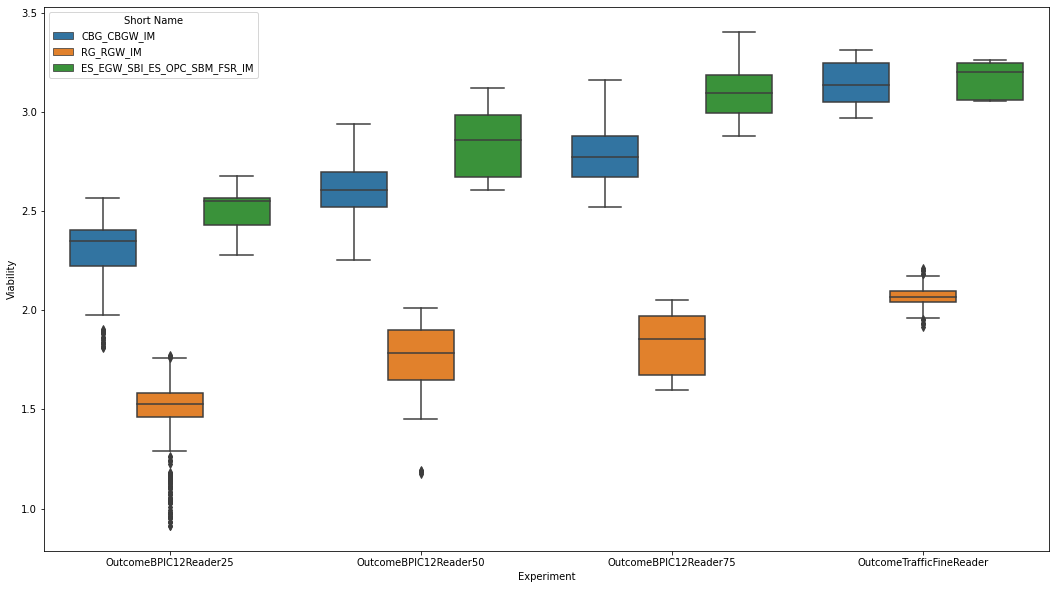
\includegraphics[width=\textwidth]{figures/generated/exp5_winner_overall.png}
    \caption{This figure shows boxplots of the viability of each models' generated counterfactual.}
    \label{fig:exp5-winner}
\end{figure}

Here, \attention{a specific model} returns an avarage viability of \attention{some value}. This result is not surprising, as we optimize with the same metric used to evaluate the results. 

% TODO
A notable observation occurs in the processing time. Although all models require more time to produce their results, if we increase the maximum length of sequences, the evolutionary algorithms require substiantially more time. \autoref{tbl:exp5_duration} shows, the processing time is much higher than the baseline models. On average, \attention{evo model} require \attention{duration in seconds}, while \attention{other models} require \attention{XX}, \attention{XX} and \attention{XX}, respectively.


\end{document}